\section{Markov Chain Monte Carlo simulations}

In this problem, we are looking at a well known data set of time intervals between successive coal-mining disasters in the UK involving ten or more killed. 

\subsection{Exploring the data set}

\subsection{The posterior distribution} \label{posterior}
We are adopting a hierarchical Bayesian model to analyse the data set. We assume that the coal-mining disasters follow a inhomogeneous Poisson Poisson process with intensity function $\lambda(t)$. We assume $\lambda(t)$ to be piecewise constant with $n$ breakpoints. We let $t_0$ and $t_{n+1}$ denote the start and the end times for the data set and let $t_k; k = 0,...,n$ denote the break points of the intensity function. We then have 
\todo{Trenger jeg ha med all denne forklaringen, eller er det nok å si at n = 1 litt tidligere?} 


\begin{align}
    \lambda(t) = 
    \begin{cases}
        \textbf{for } t \in [t_{k-1}), k = 1,...,n, \\
        \textbf{for } t \in [t_n, t_{n+1}].
    \end{cases}
\end{align}

One can derive the likelihood function for the observed data as

\begin{align}
    f(x|t_1,...,tn,\lambda_1,...,\lambda) 
    = exp \Big( - \sum_{k = 0}^n \lambda_k (t_{k-1} - t_k) \prod_{k = 0}^n \lambda_k^{y_k} \Big), 
\end{align}
where $x$ is the observed data and $y_k$ is the number of observed disasters in the period $t_k$ to $t_{k+1}$. 

We assume $t_1,...,t_n$ to be apriori uniformly distributed on the allowed values, and $\lambda_0,...,\lambda_n$ to be apriori independent of $t_1,...,t_n$ and apriori independent from each other. Apriori we also assume all $\lambda_0,...,\lambda_n$ to be distributes from the same gamma distribution with $\alpha = 2$ and scale parameter $\beta$. Thus, we have 

\begin{align}
    \pi(\lambda_i | \beta) = \frac{1}{\beta^2}\lambda_i e^{-\frac{\lambda_i}{\beta}} \textbf{ for } \lambda_i \geq 0,
\end{align}

and for $\beta$ we use the improper prior 

\begin{align}
    \pi (\beta) \propto \frac{exp\{ -\frac{1}{\beta} \} }{\beta} \textbf{ for } \beta > 0.
\end{align}

In the following we assume $n = 1$, so our model parameters are $\theta = (t_1, \lambda_0, \lambda_1, \beta)$. 

To find an expression for the posterior model for $\theta$ given $x$, $f(\theta|x)$, we use Bayes' theorem, and find that 
\todo{forklar mer hvordan vi kommer fram til dette?}
\begin{align}
    f(\theta|x) \propto f(x|\theta) \pi(\theta).
\end{align}
The likelihood $f(x | \theta)$ is given, and we need to find an expression for the apriori $\pi(\theta)$. Because of the independence between $t_1, \lambda_0$ and $\lambda_1$, as well as $\pi(t_1|\beta) = \pi(t_1)$ we have

\begin{align}
    \pi(\theta) 
    = \pi(t_1, \lambda_0, \lambda_1, \beta) \nonumber \\
    = \pi(t_1, \lambda_0, \lambda_1 | \beta) \cdot \pi(\theta) \nonumber \\
    = \pi(t_1) \cdot \pi(\lambda_0|\beta) \cdot \pi(\lambda_1|\beta) \cdot \pi(\beta).
\end{align}

So, using this and the given likelihood, we can find the posterior distribution for $f(\theta|x)$
\todo{sjekk dette uttrykket. utregningen er litt ulik Aurora sin.}
\begin{align} \label{eq:post}
    f(\theta|x) \propto exp \Big( - \sum_{k = 0}^1 \lambda_k (t_{k+1} - t_k) \Big)\cdot \prod_{k = 0}^1 \lambda_k^{y_k} \cdot \frac{1}{t_2-t_0} 
    \Big( \frac{1}{\beta^2} \lambda_0 \cdot
    exp \Big({-\frac{\lambda_0}{\beta}} \Big)  \Big) \nonumber \\ 
    \cdot \Big( \frac{1}{\beta^2} \lambda_1 \cdot exp \Big({-\frac{\lambda_1}{\beta}} \Big) \Big) \cdot exp \Big( -\frac{1}{\beta} \Big)/\beta \nonumber \\
    \propto   \frac{1}{\beta^5} \cdot \lambda_0^{y_0 + 1} \cdot \lambda_1^{y_1 + 1} \cdot exp \Big( -\frac{1}{\beta}(\lambda_0 + \lambda_1 + 1) - \lambda_0(t_1-t_0) - \lambda_1(t_2-t_1) \Big)
\end{align}


\subsection{Finding the full conditionals} \label{full_cond}

To find the full conditional for each of the elements in $\theta$, we use the expression for the posterior distribution found above in section \ref{posterior}. When we are looking at the full conditional for one of the elements in $\theta$, the other parameters stays constant. This means what we can overlook them for now, and we get that the full conditional for $t_1$ is

\begin{align}
    f(t_1 | \lambda_0, \lambda_1, \beta, x) \propto 
    \lambda_0^{y_0 + 1} \lambda_1^{y_1 + 1} \cdot exp \Big( -\lambda_0(t_1 - t_0) - \lambda_1 (t_2 - t_1) \Big) \nonumber \\
    \propto  \lambda_0^{y_0 + 1} \lambda_1^{y_1 + 1} \cdot exp \Big( -(\lambda_0 - \lambda_1)t_1 \Big).
\end{align}

We do not recognize the expression for the full conditional as belonging to a named distribution. 

The full conditional for $\lambda_0$ and $\lambda_1$ can also be found by using the posterior distribution from equation \ref{eq:post}. Thus, 

\begin{align}
    f(\lambda_0 | \lambda_1, t_1, \beta, x) \propto
    \lambda_0^{y_0 + 1}\cdot exp \Big( -\frac{1}{\beta} \lambda_0 - (t_1 - t_0)\lambda_0 \Big) 
    \nonumber \\
    \propto \frac{1}{\beta^{\alpha} \Gamma(\alpha)}\cdot \lambda_0^{y_0 + 1} \cdot exp \Big( - \lambda_0 (\frac{1}{\beta} + t_1 - t_0) \Big),
     \\
    f(\lambda_1 | \lambda_0, t_1, \beta, x) \propto
    \lambda_1^{y_1 + 1}\cdot exp \Big( -\frac{1}{\beta} \lambda_1 - (t_2 - t_1)\lambda_1 \Big) \nonumber \\
    \propto \frac{1}{\beta^{\alpha} \Gamma(\alpha)}\cdot \lambda_1^{y_1 + 1} \cdot exp \Big( - \lambda_1 (\frac{1}{\beta} + t_2 - t_1) \Big),
\end{align}
and we see that the full conditional for $\lambda_0$ and the full conditional for $\lambda_1$ are both gamma distributed. 


\todo[inline]{Feil i uttrykkene for t1 og beta}

For the last parameter $\beta$, the full conditional is

\begin{align}
    f(\beta | \lambda_0, \lambda_1, t_1, x) \propto 
    \frac{1}{\beta^5} \cdot exp \Big( -\frac{1}{\beta}(\lambda_0 + \lambda_1 + 1) \Big),
\end{align}

and we also recognize this as belonging to a gamma distribution. 

\subsection{Implementing a single site MCMC algorithm}

We have defined and implemented a single site MCMC algorithm for $f(\theta |x)$. $f(\theta|x)$ is the target distribution we want to sample from.  As the full conditionals of $\beta^i, \lambda_0^i$ and $\lambda_1^i$ belong to known distributions found in section \ref{full_cond}, we can use Gibbs sampling to draw directly from the full conditionals for these parameters. For $t_1$ however, this is not possible.
To find $t_1$, we use the Metropolis-Hastings algorithm. We draw an initial state for $t$ and then propose a new state $t_{new}$ from $Q()$, where $Q()$ is our proposal distribution. We have chosen $Q() \sim N(t_{old}, \sigma)$. We then compute the acceptance probability for $t_{new}$

\begin{align}
    \alpha() = min \Big( 1, \frac{f(t_{new}| \lambda_0, \lambda_1, \beta, x)}{f(t_{old}| \lambda_0, \lambda_1, \beta, x)} \Big) \nonumber \\ 
    = min \Big( \frac{\lambda_0^{y_0 + 1} \cdot \lambda_1^{y_1 + 1} exp(-(\lambda_0 - \lambda_1)t_{new})}{\lambda_0^{y_0 + 1} \cdot \lambda_1^{y_1 + 1} exp(-(\lambda_0 - \lambda_1)t_{old})} \Big) \nonumber \\
    = min \Big( 1, \frac{exp(-(\lambda_0 - \lambda_1)t_{new})}{exp(-(\lambda_0 - \lambda_1)t_{old})} \Big)
\end{align}




and accept or reject the proposed $\beta$. 
\todo{Bør jeg gå mer i detalj om acceptance/rejection her?}
\todo[inline]{Skriv mer om Q og RW}


\subsection{Burn-in and mixing period of the algorithm}

To evaluate the burn-in period of the algorithm, we have plotted the values of $\lambda_0, \lambda_1, t_1$ and $\beta$ for $n$ iterations of our MCMC algorithm. This is seen in figure \ref{fig:burnin_singleMH}. 


\begin{figure}
    \centering
    \begin{subfigure}[b]{0.49\textwidth}
        \centering
        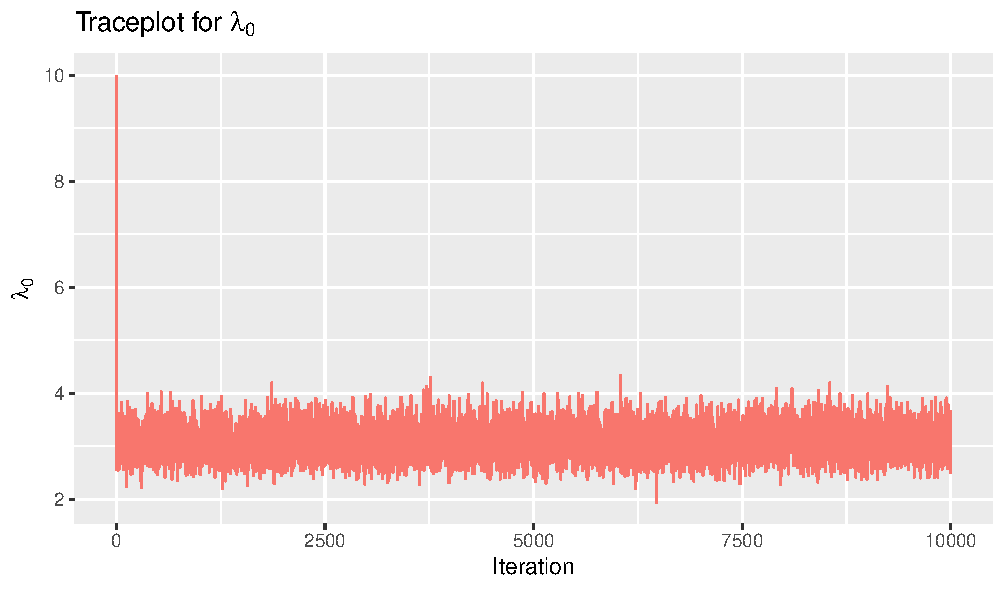
\includegraphics[width = \textwidth]{Images/sim_lambda0.pdf}
        \caption{$\lambda_0$}
        \label{fig:burnin_lam0}
    \end{subfigure}
    \begin{subfigure}[b]{0.49\textwidth}
        \centering
        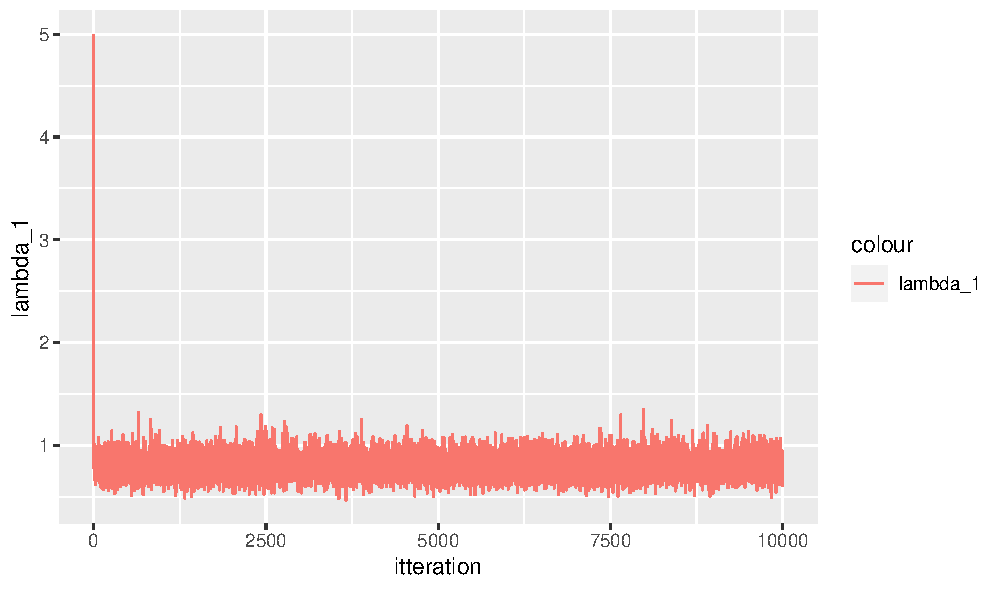
\includegraphics[width = \textwidth]{Images/sim_lambda1.pdf}
        \caption{$\lambda_1$}
        \label{fig:burnin_lam1}
    \end{subfigure}
    \begin{subfigure}[b]{0.49\textwidth}
        \centering
        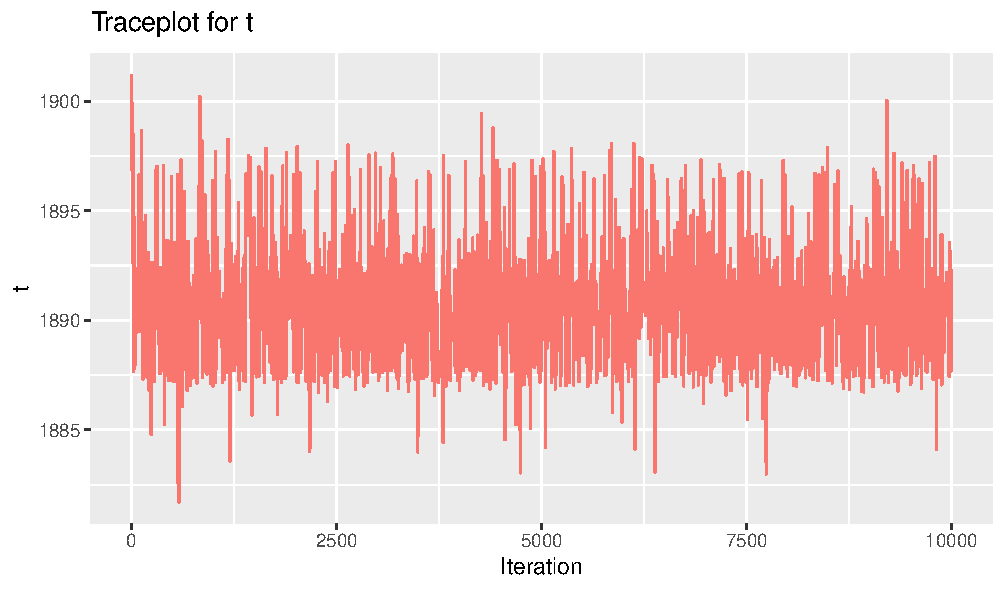
\includegraphics[width = \textwidth]{Images/sim_t.pdf}
        \caption{$t$}
        \label{fig:burnin_t}
    \end{subfigure}
    \begin{subfigure}[b]{0.49\textwidth}
        \centering
        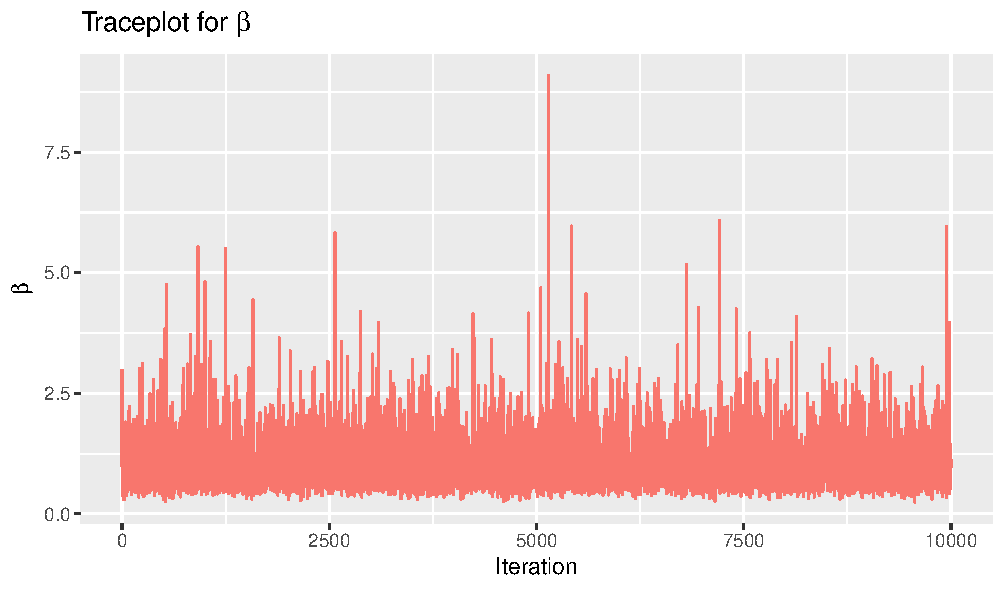
\includegraphics[width = \textwidth]{Images/sim_beta.pdf}
        \caption{$\beta$}
        \label{fig:burnin_beta}
    \end{subfigure}
    \caption{The value of $\lambda_0, \lambda_1, t$ and $\beta$ plotted for $n = 10000$ iterations of the MCMC algorithm.}
    \label{fig:burnin_singleMH}
\end{figure}

We plotted the parameters separately so they are easier to evaluate. We need to choose a burn-in period for the algorithm equal to the longest burn-in period amongst the parameters. 
In figure \ref{fig:burnin_lam0} and \ref{fig:burnin_lam1}, we see that the simulations stabilize very quickly, and there is a very small burn-in period for these parameters.
\todo[inline]{burn-in for beta. Den er ikke helt stabil}
\todo[inline]{Burn-in for t. Ikke helt stabil. Ta med plott fra forskjellige ekstremverdier av t, of forklar jvordan disse ser ut..}
For the parameter $beta$, we see that the samples fluctuate, but the mean and variance of the simulations does not seem to change. For the $t$-parameter however, we see that the mean slightly changes when the number of iterations increase. This means that we should investigate the burn-in period of this parameter more closely. 
We do this by running the algorithm $n = 50000$ and $n = 100000$ times. 

%mixing

To evaluate the mixing properties of our algorithm, we first plot the autocorrelation function for our parameter $t$ after the initial burn-in period, which we have set to be $b = *???$ iterations. The autocorrelation plot is shown in figure \ref{}. From the plot we see that the correlation decreases between the samples as the distance increases, and after $lag = 20$, there is no significant autocorrelation between the drawn samples. This indicates that the mixing is not slow. 

To investigate the mixing property further, we can 
\todo[inline]{Use the plot generated in 1 to simulate whether the simulated values are reasonable.}

\subsection{The tuning parameter and how it influences the burn-in and mixing of the simulated Markov Chain}

We have implemented our Markov Chain Monte Carlo algorithm with a tuning parameter $\sigma$. The tuning parameter is the variance for our proposal distribution $Q()$. $\lambda_0, \lambda_1$ and $\beta$ are drawn from known distributions, so the tuning parameter will not affect these samples. For our parameter $t$ however, the tuning parameter will change the acceptance rate of the algorithm. By using a small tuning parameter $\sigma$, the new proposal $t_{new}$ will be similar to the old value $t_{old}$ and the mixing will be slow. When increasing the tuning parameter, the variance in the proposal distribution is increased, and $t_{new}$ will vary more from $t_{old}$. This means that correlation between the samples decreases and the mixing increases. We cant to adjust the tuning parameter such that we get enough mixing for the algorithm to take large enough steps to explore the target density efficiently, but not so large that the acceptance rate becomes too low. We are looking for an acceptance rate of $20 - 50\%$. In figure \ref{"Set in plots with different values of sigma t"} we can see how the tuning parameter $\sigma$ affects the simulated samples of $t$.  Here we see that with $\sigma = 0.2$, the steps taken are very small. This leads to a slow exploration of the target density, and we see that $n = 10000$ iterations are far too few for the algorithm to converge. This again leads to a very large burn-in period. For $\sigma = 3$, we see that the there is enough mixing for the samples to quickly converge, and the burn-in period thus become small. If we use a very large tuning parameter, for instance $\sigma = 30$, the should be little correlation between $t_{new}$ and $t_{old}$. This means that large moves are proposed, but not often accepted. 

%Skriv noe om at stegene aksepteres mindre ofte, men fortsatt ganske ofte med sigma = 30. Skriv også hvorfor vi ikke kan ha hæyere sigma. Fordi det blir maskinelt 0 når eksponentene i e i uttrykket blir for store?

\todo[inline]{Error om vi bruker for stor sigma. Klarer ikke kjøre med f.eks sigma = 50. Se på grunner til dette. }
\todo[inline]{legg inn figurer, sigma = 0.2, sigma = 3, Sigma = 30}


\subsection{Implementing a block Metropolitan-Hastings algorithm}


\subsubsection{Using a block proposal for $(t_1, \lambda_0, \lambda_1)$ keeping $\beta$ unchanged}

\subsubsection{Using a block proposal for $\beta, \lambda_0, \lambda_1$ keeping $t_1$ unchanged}

\subsection{The block Metropolitan-Hastings algorithm for different values of the tuning parameter}